\begin{figure}
  \centering
  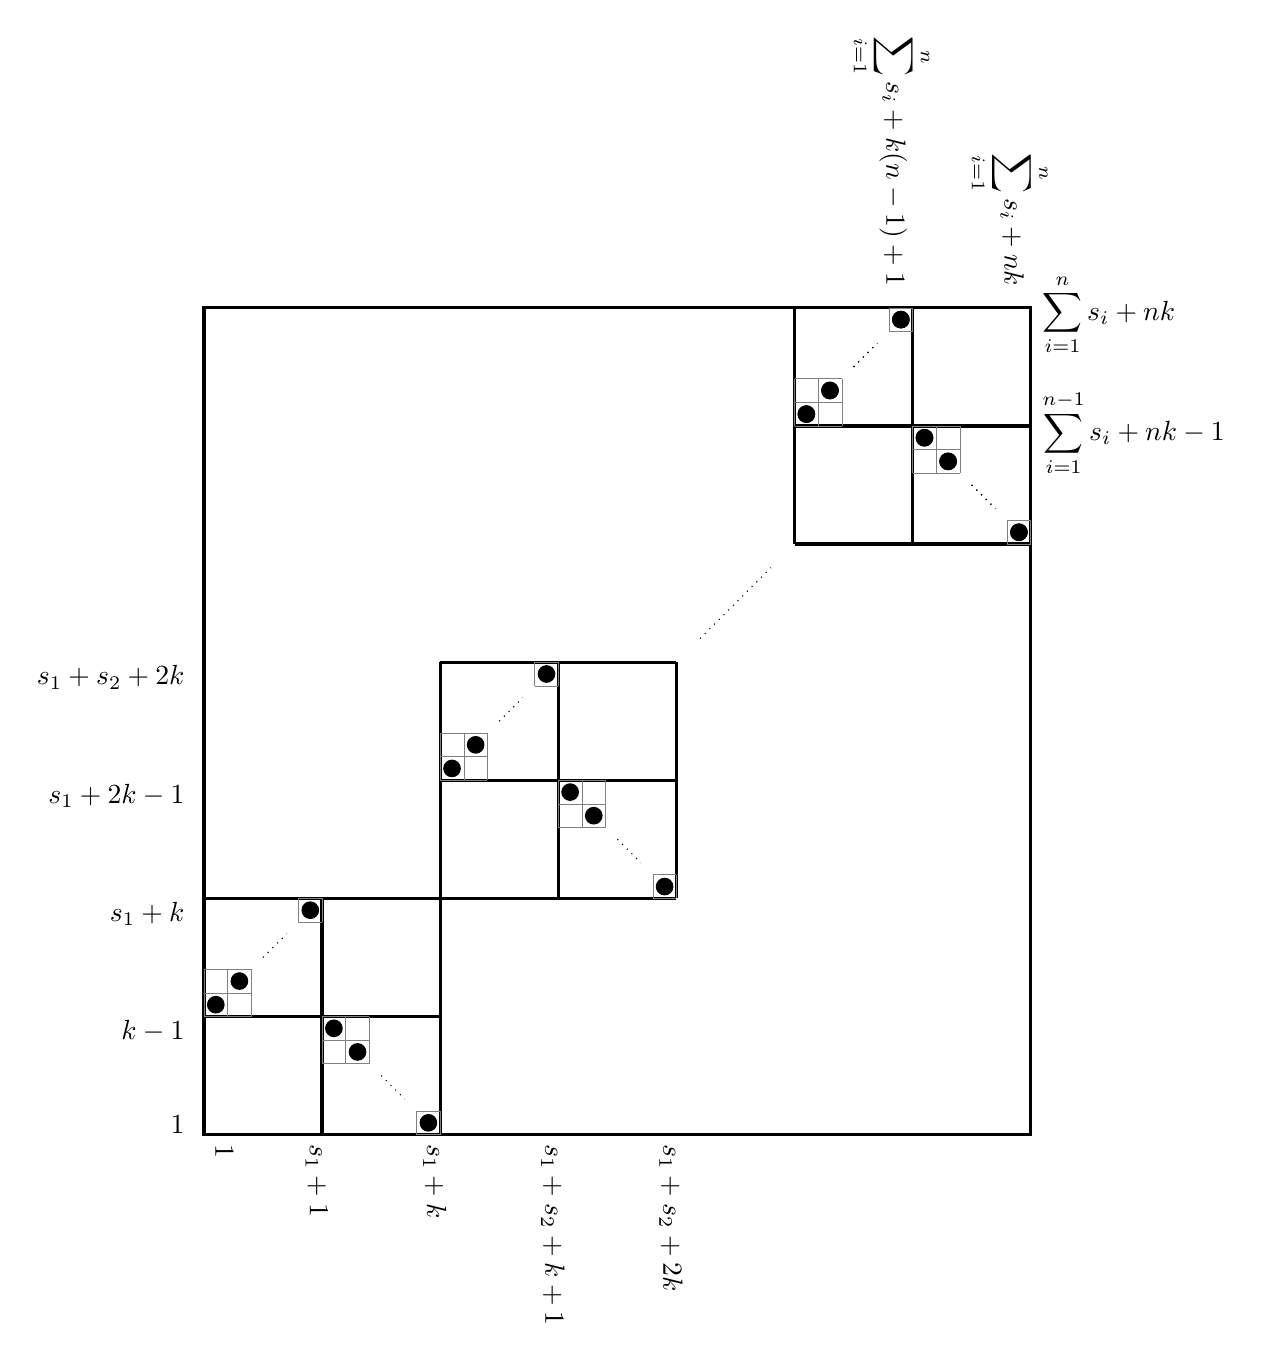
\begin{tikzpicture}
    [
      scale=.3,
    ]
    %
    \draw [black,very thick] (0, 0) rectangle (35, 35);
    \draw [step=5cm,very thick] (0, 0)   grid (10, 10);
    \draw [step=5cm,very thick] (10, 10) grid (20, 20);
    \draw [dotted] (21, 21) -- (24, 24);
    \draw [step=5cm,very thick] (25, 25) grid (35, 35);

    \foreach \x/\y in {0/0, 10/10,25,25} {
      % increasing
      \draw [black, help lines] (\x + 0, \y + 5) grid (\x + 2, \y + 7);
      \draw [black, help lines] (\x + 4, \y + 9) grid (\x + 5, \y + 10);
      \draw [black,fill=black] (\x + 1 - .5, \y + 6 -.5) circle (0.35);
      \draw [black,fill=black] (\x + 2 - .5, \y + 7 -.5) circle (0.35);
      \draw [dotted] (\x + 2.5, \y + 7.5) -- (\x + 3.5, \y + 8.5);
      \draw [black,fill=black] (\x + 5 - .5, \y + 10 -.5) circle (0.35);

      % decreasing
      \draw [black, help lines] (\x + 5, \y + 3) grid (\x + 7, \y + 5); 
      \draw [black, help lines] (\x + 9, \y + 0) grid (\x + 10, \y + 1);
      \draw [black,fill=black] (\x + 6 - .5, \y + 5 -.5) circle (0.35);
      \draw [black,fill=black] (\x + 7 - .5, \y + 4 -.5) circle (0.35);
      \draw [dotted] (\x + 7.5, \y + 2.5) -- (\x + 8.5, \y + 1.5);
      \draw [black,fill=black] (\x + 10 - .5, \y + 1 -.5) circle (0.35);
    }

    % x-labels
    \node [label={[text depth=1.75ex,label distance=0.0cm,rotate=-90]right:{$1$}}] at (0,0) {};
    \node [label={[text depth=1.75ex,label distance=0.0cm,rotate=-90]right:{$s_1+1$}}] at (4,0) {};
    \node [label={[text depth=1.75ex,label distance=0.0cm,rotate=-90]right:{$s_1+k$}}] at (9,0) {};
    \node [label={[text depth=1.75ex,label distance=0.0cm,rotate=-90]right:{$s_1+s_2+k+1$}}] at (14,0) {};
    \node [label={[text depth=1.75ex,label distance=0.0cm,rotate=-90]right:{$s_1+s_2+2k$}}] at (19,0) {};
    \node [label={[text depth=1.75ex,label distance=0.0cm,rotate=-90,anchor=east]right:{$\displaystyle\sum_{i=1}^{n}s_i+k(n-1)+1$}}] at (29,35.5) {};
    \node [label={[text depth=1.75ex,label distance=0.0cm,rotate=-90,anchor=east]right:{$\displaystyle\sum_{i=1}^{n}s_i+nk$}}] at (34,35.5) {};

    % y labels
    \node [label={[text depth=1.75ex,label distance=0.0cm,anchor=east]left:{$1$}}] at (0, 0) {};
    \node [label={[text depth=1.75ex,label distance=0.0cm,anchor=east]left:{$k-1$}}] at (0, 4) {};
    \node [label={[text depth=1.75ex,label distance=0.0cm,anchor=east]left:{$s_1+k$}}] at (0, 9) {};
    \node [label={[text depth=1.75ex,label distance=0.0cm,anchor=east]left:{$s_1+2k-1$}}] at (0, 14) {};
    \node [label={[text depth=1.75ex,label distance=0.0cm,anchor=east]left:{$s_1+s_2+2k$}}] at (0, 19) {};
    \node [label={[text depth=1.75ex,label distance=0.0cm,anchor=west]left:{$\displaystyle\sum_{i=1}^{n-1}s_i+nk-1$}}] at (35.5, 30) {};
    \node [label={[text depth=1.75ex,label distance=0.0cm,anchor=west]left:{$\displaystyle\sum_{i=1}^{n}s_i+nk$}}] at (35.5,35) {};
  \end{tikzpicture}
  \caption{\label{fig:bin-packing}%
  \textsc{Bin Packing}.}
\end{figure}
